\section{Introduction}

The visual information that we get by using our eyes can give us an idea of what objects we are looking at, but this information can also give us an idea of the distances to those objects from where we stand. In order to see how far away objects are we get visual cues which help us  process an object's location in 3D space. These are called depth cues\citep[p.~195]{sensationPerception}.\\
This essay describes some of these depth cues, which can be seen in \autoref{fig:depthCues}, and gives a few examples of how they work through figures. Furthermore, it describes some examples of how these depth cues are used in media technology.

\begin{figure}[H]
	\centering
	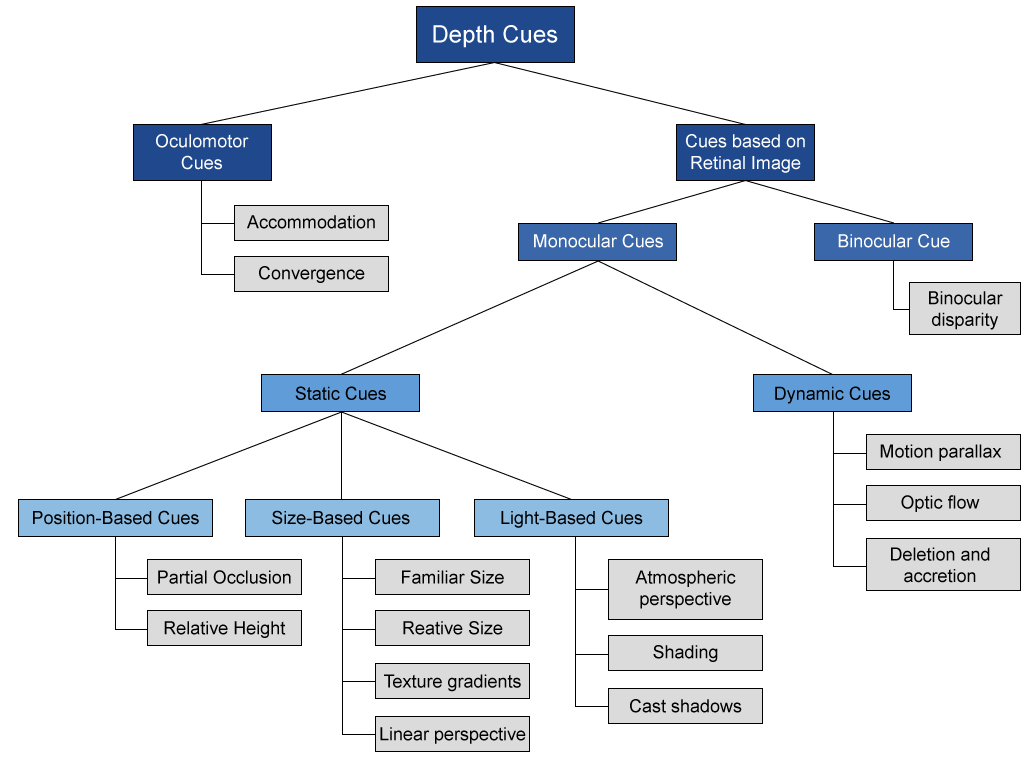
\includegraphics[width=1\linewidth]{figure/Analysis/depthCues.png}
	\caption{Model displaying the various depth cues. This model is a reconstruction of the model in the \textit{Sensation and perception} book\citep[p.~195]{sensationPerception}.}
	\label{fig:depthCues}
\end{figure}